\section{Axiale Lasermoden}

In diesem Teil beschäftigen wir uns mit den axialen Lasermoden. Dafür verwenden wir ein durchstimmbares konfokales Fabry-Pérot-Interferometer. 
Dazu führt man den Laser möglichst parallel in das Interferometer. Die vom Fabry-Pérot-Interferometer durchgelassene Intensität wird dann von einer 
Photodiode detektiert, verstärkt um einen Faktor 100 und dann grafisch dargestellt. Die Rampenspannung des Interferometers wird dann so eingestellt, 
das man 2 mal den freien Spektralbereich sieht. Dies erkennt man daran, dass man genau zwei mal das gleiche Bild nebeneinander auf dem Oszilloskop sieht. 
Den Abstand der Lasermoden bestimmen wir einfach durch Ablesen am Oszilloskop. Zuvor müssen wir aber herausfinden, wie das Zeitsignal auf der 
x-Achse des Oszilloskops mit der Frequenz zusammenhängt.\\

Dazu nehmen wir zwei mal den selben Peak, aber in zwei nebeneinanderliegenden Darstellungen auf Channel 1 in Abbildung \ref{bild:FreierSpektralbereich}.
Dieser Abstand entspricht dem freien Spektralbereich des Interferometers. Dieser ist bei dem hier verwendeten Gerät 2\,GHz. Man könnte ebenfalls das Triggersignal verwenden, 
aber an den Peaks kann man das Maximum leichter ablesen. Man erhält also den Umrechnungsfaktor 

\begin{equation*}
    m = (152 \pm 7)\,\frac{\mathrm{MHz}}{\mathrm{ms}}
\end{equation*}

für die Umrechnung 

\begin{equation}
    \Delta \nu = m\cdot \Delta t
    \label{eq:Umrechnung}
\end{equation}

von der vom Oszilloskop ausgegebenen Zeitdifferenz in Frequenzen $\nu$.


\begin{figure}[ht]
    \centering
    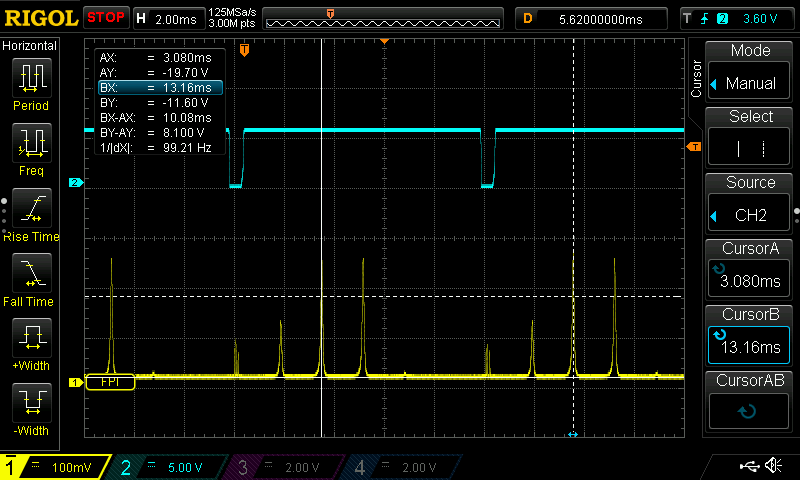
\includegraphics[width = \linewidth]{Bilder/Auswertung/FabryPerotKalibr.png}
    \caption{Longitudinale Lasermoden mit dem Fabry-Pérot aufgenommen. Channel 1 ist das Messsignal und Channel 2 ist des Triggersignal des Interfermoters. Gekennzeichnet sind 
    mit den x-Marker zwei gleich Peaks.}
    \label{bild:FreierSpektralbereich}
\end{figure}


\subsection*{Abstand und Linienbreite Axialer Lasermoden}

Den Abstand der Moden bestimmt man auch grafisch aus Abbildung \ref{bild:AxialModenAbstand}. Aus diesem erhält man 
\begin{equation*}
    \Delta t = (1,660 \pm 0,086)\,\mathrm{ms}
\end{equation*}
und mit der Umrechnung aus Gleichung \ref{eq:Umrechnung} erhalt man 

\begin{equation}
    \textcolor{red}{\Delta \nu_{Modenabstand} = (252 \pm 17)\,\mathrm{MHz}}
    \label{eq:Modenabstand}
\end{equation}

den Abstand zweier longitudinaler Lasermoden. Die Unsicherheit wird hierbei aus geschätzter Ableseunsicherheit und
der Unsicherheit der Kalibrierung  mittels Fehlerfortpflanzung berechnet. Auf selbe Weise wird 

\begin{equation}
    \textcolor{red}{\Delta \nu_{Linienbreite} = (13,3 \pm 1,5)\,\mathrm{MHz}}
\end{equation}

auch die Linienbreite aus Abbildung \ref{bild:Lininebreite} bestimmt.

\begin{figure}[ht]
    \centering
    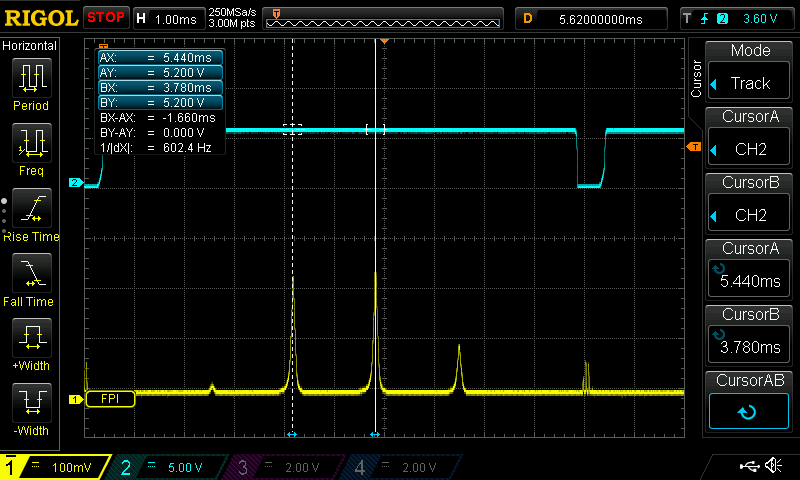
\includegraphics[width = \linewidth]{Bilder/Auswertung/FabryPerotModenAbstand.png}
    \caption{Longitudinale Lasermoden mit dem Fabry-Pérot aufgenommen. Mit den x-Markern wird der Abstand zweiter Lasermoden $\Delta \nu_{Modenabstand}$ bestimmt. Dieser muss aber noch in Hz umgerechnet werden.}
    \label{bild:AxialModenAbstand}
\end{figure}

\begin{figure}[ht]
    \centering
    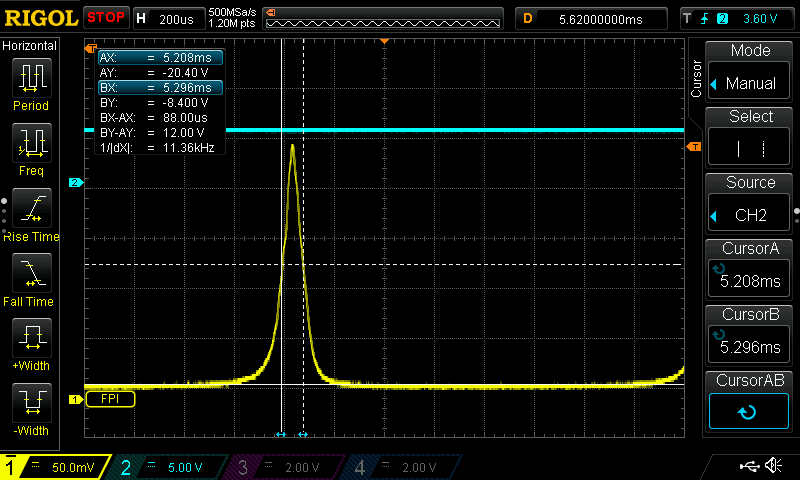
\includegraphics[width = \linewidth]{Bilder/Auswertung/FabryPerotLinienbreite.png}
    \caption{Longitudinale Lasermoden mit dem Fabry-Pérot aufgenommen. Mit den x-Markern wird die Lininebreite $\Delta \nu_{Linienbreite}$ bestimmt. Dieser muss aber noch in Hz umgerechnet werden.}
    \label{bild:Lininebreite}
\end{figure}